\documentclass[UTF8]{ctexart}
\usepackage{amsmath}
\usepackage{amssymb}
\usepackage{background}
\usepackage{booktabs}
\usepackage{enumitem}
\usepackage{fancyhdr}
\usepackage{float}
\usepackage{fontspec}
\usepackage{geometry}
\usepackage{listings}
\usepackage{multirow}
\usepackage{tabularx}
\usepackage{tasks}
\usepackage{tcolorbox}
\tcbuselibrary{breakable}
\usepackage{tikz}
\usetikzlibrary{arrows.meta, positioning, calc}
\usepackage[table]{xcolor}

\geometry{a5paper, top=0.1cm, left=1cm, right=1cm, bottom=1cm, footskip=0.1cm}
\setCJKmainfont[BoldFont={汉仪文黑-85W},ItalicFont={汉仪文黑-55W}]{汉仪文黑-55W}
\setfontfamily\Issue{Century Schoolbook}
\setfontfamily\Genshin{Genshin Teyvat Lingua Franca}
\newCJKfontfamily\TitleFont{思源宋体 CN Heavy}
\newfontfamily\timesnewroman{Times New Roman}

%————————————————可变部分——————————————————
\settasks{label={\Alph*.\ }, label-format={\color{cyan!50!black}}, item-format={\color{cyan!50!black}}}
\newcommand\col[1]{\textcolor{green!50!black}{#1}}
\newcommand\coll[1]{\textcolor{blue}{#1}}
\newcommand\dotting{\ .\ }
%\setlist[enumerate]{itemsep=0pt, parsep=0pt}
%\setlist[itemize]{itemsep=0pt, parsep=0pt}

\newcommand\FIRST{\textsc{First}}
\newcommand\FOLLOW{\textsc{Follow}}
\newcommand\NULLABLE{\textsc{Nullable}}
\newcommand\FIRSTS{\textsc{First\_s}}
\newcommand\ACTION{\textsc{Action}}
\newcommand\GOTO{\textsc{Goto}}
\newcommand\D{\text{\textbullet}}
%——————————————————————————————————————————

\pagestyle{fancy}
\fancyhf{}
\cfoot{\sffamily\footnotesize{-\ \thepage\ -}}
%

\colorlet{darkcyan}{cyan!50!black}
\newcommand\Black[1]{\textcolor[gray]{0.3}{#1}}
\newcommand\Brown[1]{\textcolor[HTML]{998A4E}{#1}}
\newcommand\Emph[1]{\colorbox{green!10}{\textcolor{green!30!black}{#1}}}
\newcommand\Notes[1]{\textcolor{yellow!50!black}{\small #1}}
\newcommand\Example[1]{\textcolor{cyan!70!black}{\small #1}}
\colorlet{note}{yellow!70!black}


\newcommand\IssueNumber{46}
\newcommand\Date{2024-12-19}
%\newcommand\Contributer{@金光日}
\newcommand\Subject{编译原理}
%\newcommand\Source{历年考研 408 真题}


\begin{document}
\backgroundsetup{contents=
\includegraphics{上半示例.png}, center, scale=1, angle=0, opacity=1}
\BgThispage
\begin{center}
%{\scriptsize\Issue \textcolor[HTML]{C8BA83}{\Genshin WEEKLY TIPS}}
\phantom{...}

{\Large\textcolor{brown!40!white}{\makebox[10cm][s]{\Genshin WEEKLY KNOWLEDGE TIPS}}}

\vspace{-2em}

{\Huge\bfseries\TitleFont \Black{知\ 识\ 小\ 料}}


\vspace{-0.1cm}
{\footnotesize \Brown{「电计 2203 班」周常规知识整理共享}}
\end{center}

\vspace{-0.5cm}


\begin{figure}[H]
\hspace{1cm}
\begin{minipage}[t]{0.3\textwidth}
\centering
    \Brown{\Genshin ISSUE}

    \vspace{-0.6cm}
    \Huge \Issue\slshape\bfseries\Black{\IssueNumber}
\end{minipage}
\hfill
\begin{minipage}[t]{0.28\textwidth}
\centering
    \Brown{日期:\Date} \\
%\vspace{-0.1cm}
%    \Brown{贡献者:\Contributer} \\
\vspace{-0.1cm}
    \Brown{学科:\Subject} \\
%\vspace{-0.1cm}
%    \Brown{来源:\Source}
\end{minipage}
\hspace{0.8cm}
\end{figure}

{\color{cyan!50!black}
已知文法 $G[S]$:
\begin{align*}
  S & \to Sf \ |\  fAk \\
  A & \to eSf \ |\  eSh \ |\  \varepsilon
\end{align*}
\begin{enumerate}[itemsep=0pt,parsep=0pt,label=(\theenumi)]
  \item 写出拓广文法,并将下图识别活前缀的 DFA 补充完整。
  \item 求出 $S,A$ 的 \FIRST 集和 \FOLLOW 集。
  \item 该文法是 LR(0) 文法吗?是 SLR(1) 文法吗?说明理由(指出 (1) 中的 LR(0) 项目集规范族是否有冲突?如果有冲突,哪个项目集存在何种冲突?)。判断后构造出相应的 SLR(1) 分析表。
\end{enumerate}
\begin{figure}[htb]
  \centering
  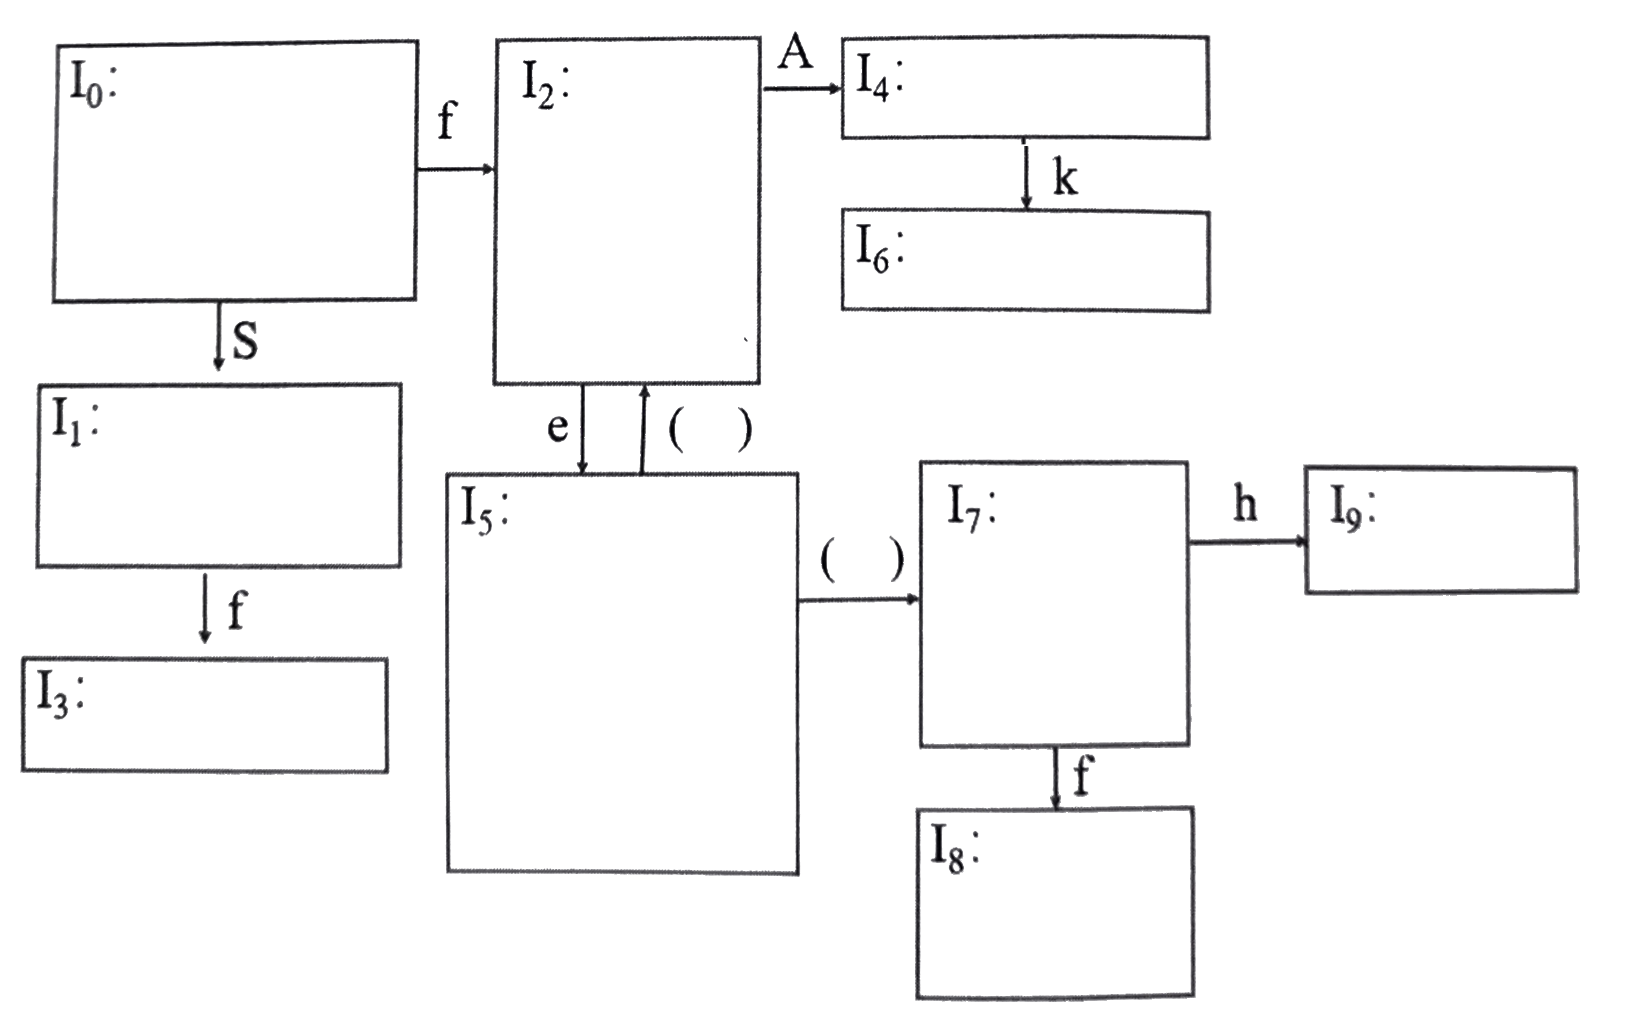
\includegraphics[width=8cm]{题目.png}
\end{figure}
}

\paragraph{第 (1) 问} 几个概念:

\begin{tcolorbox}[colback=violet!5, colframe=violet, boxrule=1pt, breakable]
\begin{description}
    \item[拓广文法] 对原有的以 $S$ 为开始符的文法 $G[S]$,增加产生式 $S'\to S\$ $\textcolor{cyan}{(教材和资料中多采用 $S'\to S$ 的产生式)},得到的新文法 $G'[S']$ 为「拓广文法」。易知拓广文法与原文法等价。
    \item[DFA] 指确定性的有穷自动机。
    \item[LR(0)项目] 在每个产生式的右部添加圆点以构成项目。比如产生式 $S\to ab$ 对应三个项目:$S\to \D ab$、$S\to a\D b$、$S\to ab\D$。特别地,空产生式 $S\to\varepsilon$ 只对应\textcolor{red}{一个项目}:$S\to\D$。
\end{description}
\end{tcolorbox}

\backgroundsetup{contents=
\includegraphics{空白示例.png}, center, scale=1, angle=0, opacity=1}
\BgThispage

原文法的拓广文法 $G'[S']$ 为:
\begin{align*}
  S' & \to S\$ \\
  S & \to Sf \ |\  fAk \\
  A & \to eSf \ |\  eSh \ |\  \varepsilon
\end{align*}

在补充 DFA 时,若遇到了形如 $S\to\D A\dots$ 的产生式(圆点紧接着非终结符),则需要把所有以该非终结符 $A$ 开头的产生式也加入到 DFA 的同一状态中。得到的 DFA 图如下:

\begin{figure}[htb]
    \centering
    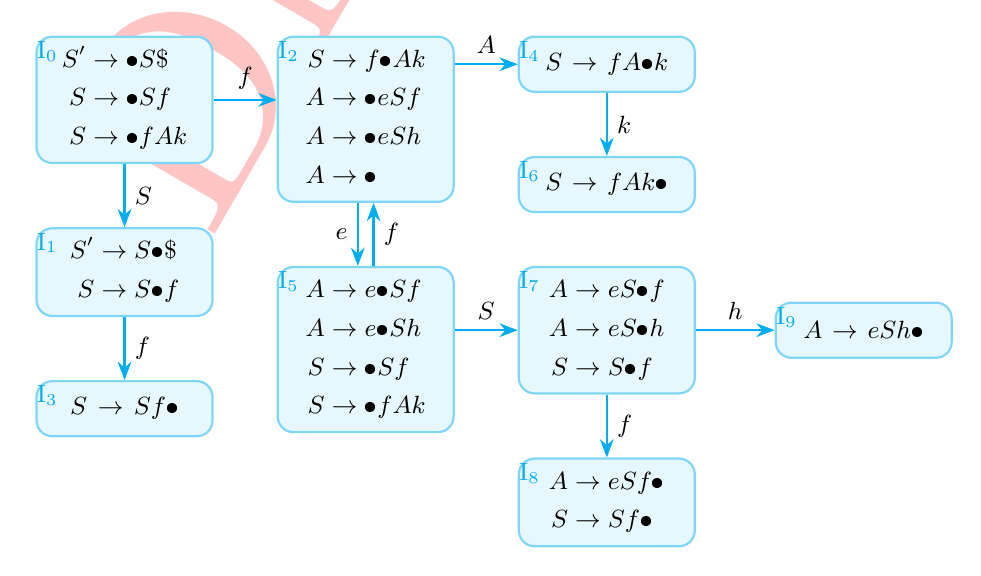
\begin{tikzpicture}[
        item/.style = {rectangle, thick, rounded corners=2mm, minimum size=0.7cm, text width=2cm, align=center, fill=cyan!10, draw=cyan!50},
        line/.style = {->, thick, cyan},
        node distance=0.8cm and 1cm, % 设置水平和垂直距离
        font = \small,
        >=Stealth,
    ]
        \node[item, anchor=north] (I0) at (0,0) {$\begin{aligned}
            S' &\to \D S\$ \\
            S &\to \D Sf \\
            S &\to \D fAk\end{aligned}$};
        \node[item, below=of I0] (I1) {$\begin{aligned}
            S' &\to S \D \$ \\
            S &\to S \D f \end{aligned}$};
        % 创建一个与I0顶部对齐的辅助结点
        \coordinate[above=0cm of I0] (I0-top);
        % 将I2定位在辅助结点的右侧,并设置其顶部与辅助结点对齐
        \node[item, anchor=north west, at={(I0-top -| I0.east)}, xshift=0.8cm] (I2) {$\begin{aligned}
            S &\to f \D Ak \\
            A &\to \D eSf \\
            A &\to \D eSh \\
            A &\to \D \end{aligned}$};
        \node[item, below=of I1] (I3) {$S\to Sf\D$};
        \node[item, anchor=north west, at={(I0-top -| I2.east)}, xshift=0.8cm] (I4) {$S\to fA\D k$};
        \node[item, anchor=north, below=of I2] (I5) {$\begin{aligned}
            A &\to e\D Sf \\
            A &\to e\D Sh \\
            S &\to \D Sf \\
            S &\to \D fAk \end{aligned}$};
        \node[item, below=of I4] (I6) {$S\to fAk\D$};
        \coordinate[above=0cm of I5] (I5-top); % 如法炮制
        \node[item, anchor=north west, at={(I5-top -| I5.east)}, xshift=0.8cm] (I7) {$\begin{aligned}
            A &\to  eS\D f \\
            A &\to  eS\D h \\
            S &\to S\D f \\
           \end{aligned}$};
        \node[item, below=of I7] (I8) {$\begin{aligned}
            A &\to eSf\D \\
            S &\to Sf \D \\
         \end{aligned}$};
        \node[item, right=of I7] (I9) {$A\to eSh\D$};
        \foreach \n in {0,1,...,9}{
            \node[xshift=0.15cm, yshift=-0.2cm, color=cyan, font=\small] at (I\n.north west) {$\mathrm{I_\n}$};
        }
        %定义辅助点
        \coordinate (T0) at ($(I0.east) + (0.8cm, 0)$);
        \coordinate (T1) at ($(I4.west) + (-0.8cm, 0)$);
        \coordinate (T2) at ($(I7.west) + (-0.8cm, 0)$);

        \draw [line] (I0) -- (I1) node[midway, right, text=black] {$S$};
        %\draw [line] (I0) -- (I2) node[midway, above] {$f$}; 替换为如下语句
        \draw [line] (I0) -- (T0) node[midway, above, text=black] {$f$};
        \draw [line] (I1) -- (I3) node[midway, right, text=black] {$f$};
        \draw [line] (T1) -- (I4) node[midway, above, text=black] {$A$};
        \draw [line] ($(I2.south)+(-0.1cm,0)$) -- ($(I5.north)+(-0.1cm,0)$) node[midway, left, text=black] {$e$};
        \draw [line] ($(I5.north)+(0.1cm,0)$) -- ($(I2.south)+(0.1cm,0)$) node[midway, right, text=black] {$f$};
        \draw [line] (I4) -- (I6) node[midway, right, text=black] {$k$};
        \draw [line] (T2) -- (I7) node[midway, above, text=black] {$S$};
        \draw [line] (I7) -- (I8) node[midway, right, text=black] {$f$};
        \draw [line] (I7) -- (I9) node[midway, above, text=black] {$h$};
    \end{tikzpicture}
    \caption{DFA 状态图}\label{fig:DFA}
\end{figure}

需要记得将括号里的转移字符补全。

\paragraph{第 (2) 问} 求 \FIRST 集和 \FOLLOW 集,参考「知识小料」·其三十七,其中有详细步骤。这里对拓广文法 $G'$ 进行处理,为了在 \FOLLOW 集得到 \$,以备后续操作。比较简单。

易知,$\NULLABLE = \{A\}$。

\begin{itemize}[itemsep=0pt,parsep=0pt]
  \item $\FIRST(S) = \{f\}$;
  \item $\FIRST(A) = \{e\}$。
\end{itemize}

\begin{itemize}[itemsep=0pt,parsep=0pt]
  \item $\FOLLOW(S) = \{f,h,\$\}$;
  \item $\FOLLOW(A) = \{k\}$。
\end{itemize}

\paragraph{第 (3) 问} 询问是否为 LR(0)、SLR(1) 文法,需要先明确概念。

\begin{tcolorbox}[colback=violet!5, colframe=violet, boxrule=1pt, breakable]
\begin{description}
    \item[移进—归约冲突] 对于某一状态,例如题中的 $\mathrm{I_2}$,若其既可对应移进操作,也可对应归约操作,则存在冲突。
    \item[归约—归约冲突] 对于某一状态,例如题中的 $\mathrm{I_8}$,若存在多个归约项目,且对应的产生式不同,则存在冲突。
    \item[LR(0)文法] 当 DFA 状态图中不存在移进—归约冲突和归约—归约冲突,则文法是 LR(0) 文法。
    \item[SLR(1)文法] 当 DFA 状态图中不存在上述两种冲突,或者虽存在冲突但可以利用 \FOLLOW 集来消解,则文法是 SLR(1) 文法。此时需要考虑前看符号(即 \FOLLOW 集的符号)。
    \item[两种文法的关系] 一个文法若为LR(0)文法,则它一定是SLR(1)文法的候选者,但反之不然。
    \item[项目集规范族] 指同一状态的 LR(0) 项目集合,如 $\mathrm{I_0}$ 的三条项目的集合。
\end{description}
\end{tcolorbox}

查看 DFA 状态图,发现状态 $\mathrm{I_2}$ 的 4 个项目中,前 3 个项目 $S\to f\D Ak$、$A\to \D eSf$、$A\to \D eSh$ 对应移进操作,而后 1 个项目 $A\to\D$ 对应归约操作,因此在这一状态下不能确定是移进 $e$ 还是归约为 $A$。据此得知,项目集 $\mathrm{I_2}$ 存在\textcolor{red}{移进—归约冲突}。

查看 DFA 状态图,还会发现状态 $\mathrm{I_8}$ 的 2 个项目中,项目 $A\to eSf\D$、$S\to Sf\D$ 分别对应于产生式 $A\to eSf$、$S\to Sf$ 的归约操作,因此在这一状态下不能确定是归约为 $A$ 还是归约为 $S$。据此得知,项目集 $\mathrm{I_8}$ 存在\textcolor{red}{归约—归约冲突}。

因此,原文法不是 LR(0) 文法。但这种情况可以用 \FOLLOW 集处理,可以试着使用 SLR(1) 分析方法填表,再判断是否是 SLR(1) 文法。

在 SLR(1) 文法中,只有归约操作与 LR(0) 文法不同:对于状态 $\mathrm{I}_i$ 的项目 $X\to \cdots\D$,仅对 $y\in \FOLLOW(X)$ 添加 $\ACTION[i,y]$ 为需要归约的产生式编号。\textcolor{cyan}{(也就是说,只有当面临 $X$ 的前看符号时,才能做出归约操作,否则报错。)}

为了便于归约,这里把拓广文法 $G'[S']$ 产生式展开写,并编号:
\begin{align*}
    0: & S'\to S\$ \\
    1: & S\to Sf \\
    2: & S\to fAk \\
    3: & A\to eSf \\
    4: & A\to eSh \\
    5: & A\to\varepsilon \\
\end{align*}

\begin{table}[htb]
    \centering
    \begin{tabularx}{0.8\textwidth}{|*{8}{X|}} % 8列等宽表格
    \hline
        \multirow{2}*{状态} & \multicolumn{5}{c|}{\ACTION 表} & \multicolumn{2}{c|}{\GOTO 表} \\
    \cline{2-8}
                       & $e$   & $f$   & $h$   & $k$   & \$    & $S$   & $A$ \\
    \hline
        $\mathrm{I_0}$ &       & $s_2$ &       &       &       & $g_1$ &       \\
    \hline
        $\mathrm{I_1}$ &       & $s_3$ &       &       & Acc.  &       &       \\
    \hline
        $\mathrm{I_2}$ & $s_5$ &       &       & \textcolor{darkcyan}{$r_5$} &       &       & $g_4$ \\
    \hline
        $\mathrm{I_3}$ &       & \textcolor{darkcyan}{$r_1$} & \textcolor{darkcyan}{$r_1$} &       & \textcolor{darkcyan}{$r_1$} &       &       \\
    \hline
        $\mathrm{I_4}$ &       &       &       & $s_6$ &       &       &       \\
    \hline
        $\mathrm{I_5}$ &       & $s_2$ &       &       &       & $g_7$ &       \\
    \hline
        $\mathrm{I_6}$ &       & \textcolor{darkcyan}{$r_2$} & \textcolor{darkcyan}{$r_2$} &       & \textcolor{darkcyan}{$r_2$} &       &       \\
    \hline
        $\mathrm{I_7}$ &       & $s_8$ & $s_9$ &       &       &       &       \\
    \hline
        $\mathrm{I_8}$ &       & \textcolor{darkcyan}{$r_1$} & \textcolor{darkcyan}{$r_1$} & \textcolor{darkcyan}{$r_3$} & \textcolor{darkcyan}{$r_1$} &       &       \\
    \hline
        $\mathrm{I_9}$ &       &       &       & \textcolor{darkcyan}{$r_4$} &       &       &       \\
    \hline
    \end{tabularx}
    \caption{SLR(1)分析表}\label{tab:SLR(1)}
\end{table}

详细说明分析表的几处:
\begin{itemize}
\renewcommand\theenumi{\roman{enumi}} % 暂时修改列表的标签为罗马数字
  \item 移进项 $s_i,g_i$ 的下标 $i$ 表示状态号 $\mathrm{I}_i$,归约项 \textcolor{darkcyan}{$r_j$} 的下标 $j$ 表示产生式号。
  \item 举例说明:对于 \textcolor{darkcyan}{$r_5$} 这一格,因为状态 $\mathrm{I_2}$ 的归约项目 $A\to\D$ 的产生式左部为 $A$,$\FOLLOW(A)=\{k\}$,所以在第 $\mathrm{I_2}$ 行仅对 $k$ 列添加 $\ACTION[2,k]$,对应的产生式是 $[5:A\to\varepsilon]$,所以填写 \textcolor{darkcyan}{$r_5$}。\textcolor{cyan}{(如果按照 LR(0) 分析法,那么 \ACTION 表部分的每一列都要填写 $r_5$。)}
  \item 举例说明:状态 $\mathrm{I_8}$ 这一行,存在归约—归约冲突。

  \begin{enumerate}[label=\theenumi)]
    \item 对项目 $A\to eSf\D$,$\FOLLOW(A)=\{k\}$,仅对 $k$ 列添加 $\ACTION[8,k]=\textcolor{darkcyan}{r_3}$(用 3 号产生式归约);
    \item 对项目 $S\to Sf\D$,$\FOLLOW(S)=\{f,h,\$ \}$,对 $f,h,\$ $ 列均需要添加 $\ACTION[8,f]=\ACTION[8,h]=\ACTION[8,\$]=\textcolor{darkcyan}{r_1}$(用1号产生式归约)。
  \end{enumerate}

  \textcolor{cyan}{(事实上,本例满足 $\FOLLOW(S)\cap \FOLLOW(A) = \varnothing$。如果不满足这一条件,那么需要在同一个单元格内填写多个归约,此时冲突无法解决,就不是 SLR(1) 文法了。)}
  \item Acc.是「接受」(Accept)的意思。
  
  \item 在分析 \FOLLOW 集时需要用拓广文法 $G'$,这是为了使原开始符 $S$ 的 \FOLLOW 集包含终结符 \$,以将 \ACTION 表的 \$ 列恰当补全。
\end{itemize}

填写分析表后,发现分析表内无冲突($\FOLLOW(S)\cap \FOLLOW(A) = \varnothing$ 这一条件立大功)。所以原文法是 SLR(1) 文法。


\vspace{1em}

{\color{cyan!80!black}
【结论】
\begin{enumerate}[itemsep=0pt,parsep=0pt,label=(\theenumi)]
    \item 拓广文法见解析,DFA 状态图如图 \ref{fig:DFA} 所示。
    \item $S,A$ 的 \FIRST 集分别为 $\{f\}$、$\{e\}$;\FOLLOW 集分别为 $\{f,h,\$ \}$、$\{k\}$。
    \item 该文法不是 LR(0) 文法,是 SLR(1) 文法,题 (1) 中的项目集规范族 $\mathrm{I_2}$ 存在移进—归约冲突,$\mathrm{I_8}$ 存在归约—归约冲突。SLR(1)分析表如表 \ref{tab:SLR(1)} 所示。
\end{enumerate}

【点评】这是一道编译原理的大题,考察了 LR(0) 和 SLR(1) 文法的分析方法。此题需要同学们会补充 DFA 状态图,会填写 \ACTION 表和 \GOTO 表,以及进行一些分析。
}

\backgroundsetup{contents=
\includegraphics{下半示例.png}, center, scale=1, angle=0, opacity=1}
\BgThispage


\end{document} 